\chapter{Cronograma} 

\begin{table}[htpb]
\begin{center}
\caption{Cronograma geral.}
\begin{tabular}{|c|c|c|}
\hline
\textbf{Geral}          & \textbf{Previsto} & \textbf{Realizado} \\ \hline
Início do projeto       & 30/03/2026        & 01/04/2026         \\ \hline
Fim do projeto          & 24/06/2026        & xx/xx/2026         \\ \hline
\end{tabular}
\end{center}
\end{table}

\begin{landscape}
\begin{figure}[H]
    \centering
    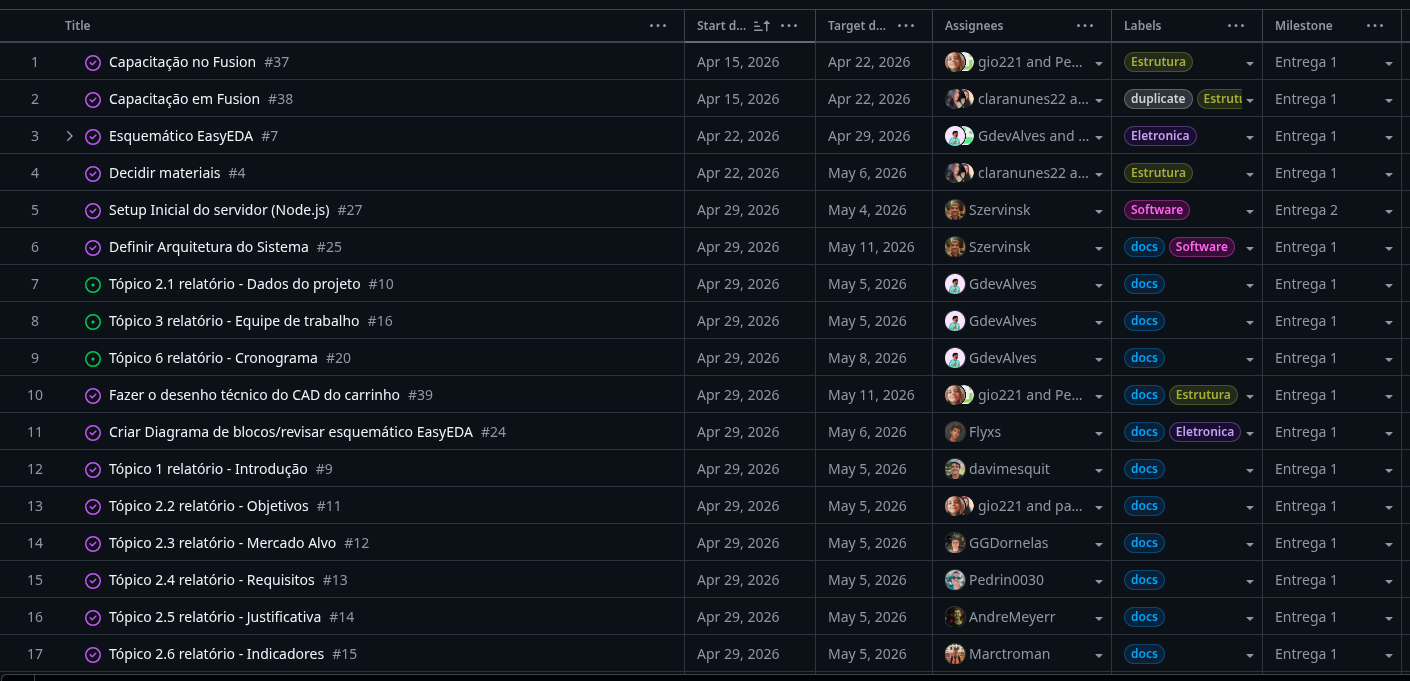
\includegraphics[width=\linewidth]{figuras/1-17.png}
    \caption{}
    \label{fig:cronograma_1_17}
\end{figure}
\end{landscape}

\begin{landscape}
\begin{figure}[H]
    \centering
    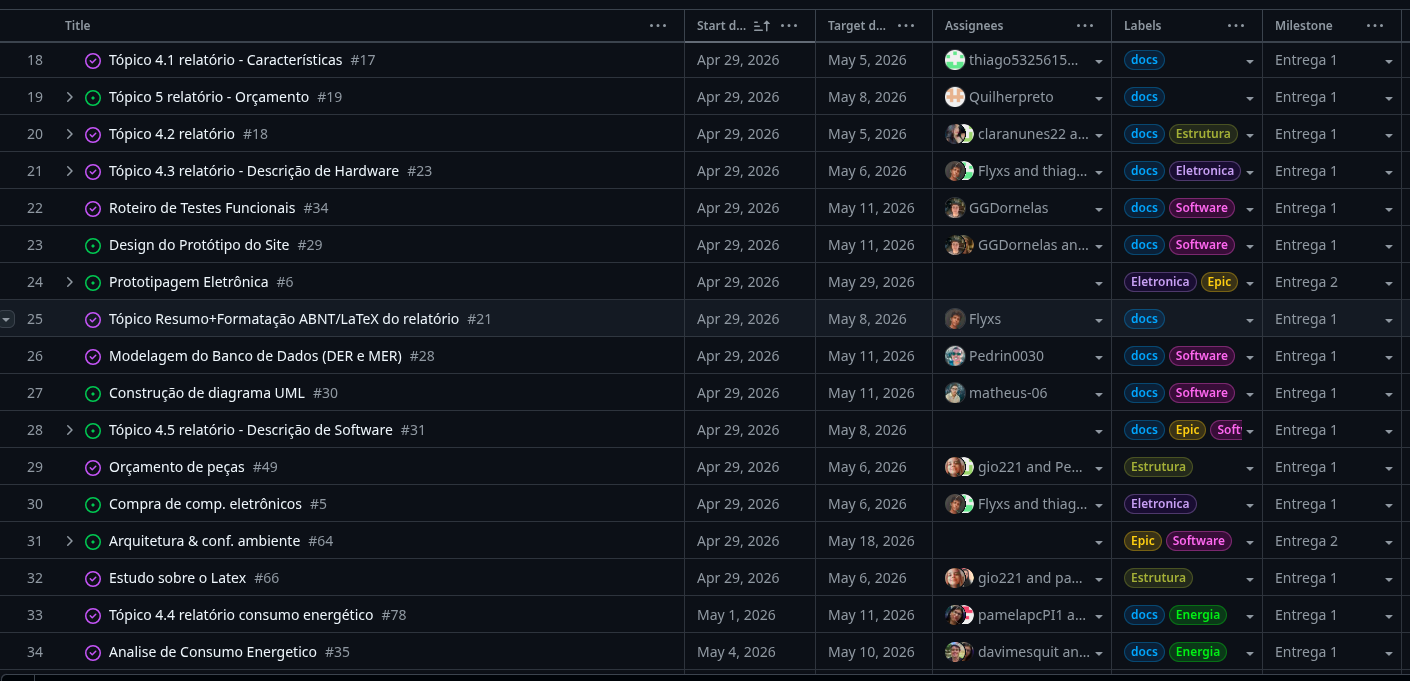
\includegraphics[width=\linewidth]{figuras/18-34.png}
    \caption{}
    \label{fig:cronograma_18_34}
\end{figure}
\end{landscape}

\begin{landscape}
\begin{figure}[H]
    \centering
    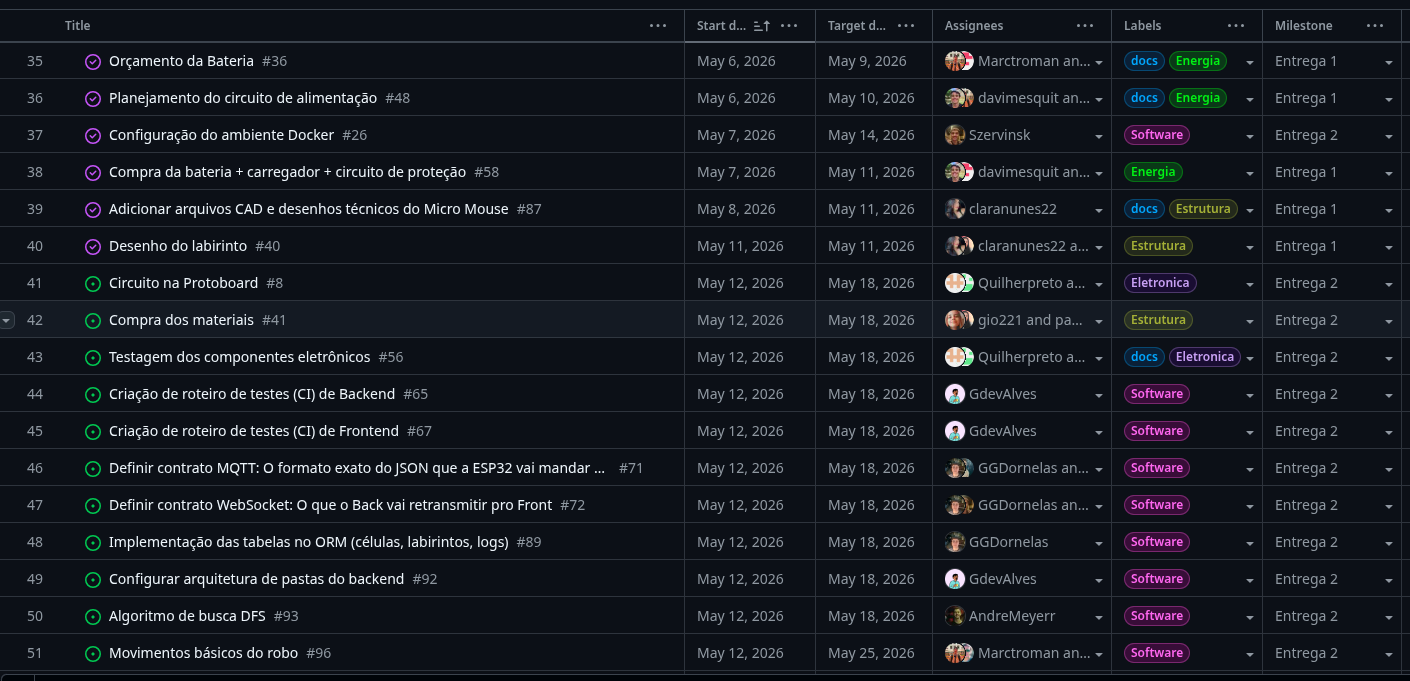
\includegraphics[width=\linewidth]{figuras/35-51.png}
    \caption{}
    \label{fig:cronograma_35_51}
\end{figure}
\end{landscape}

\begin{landscape}
\begin{figure}[H]
    \centering
    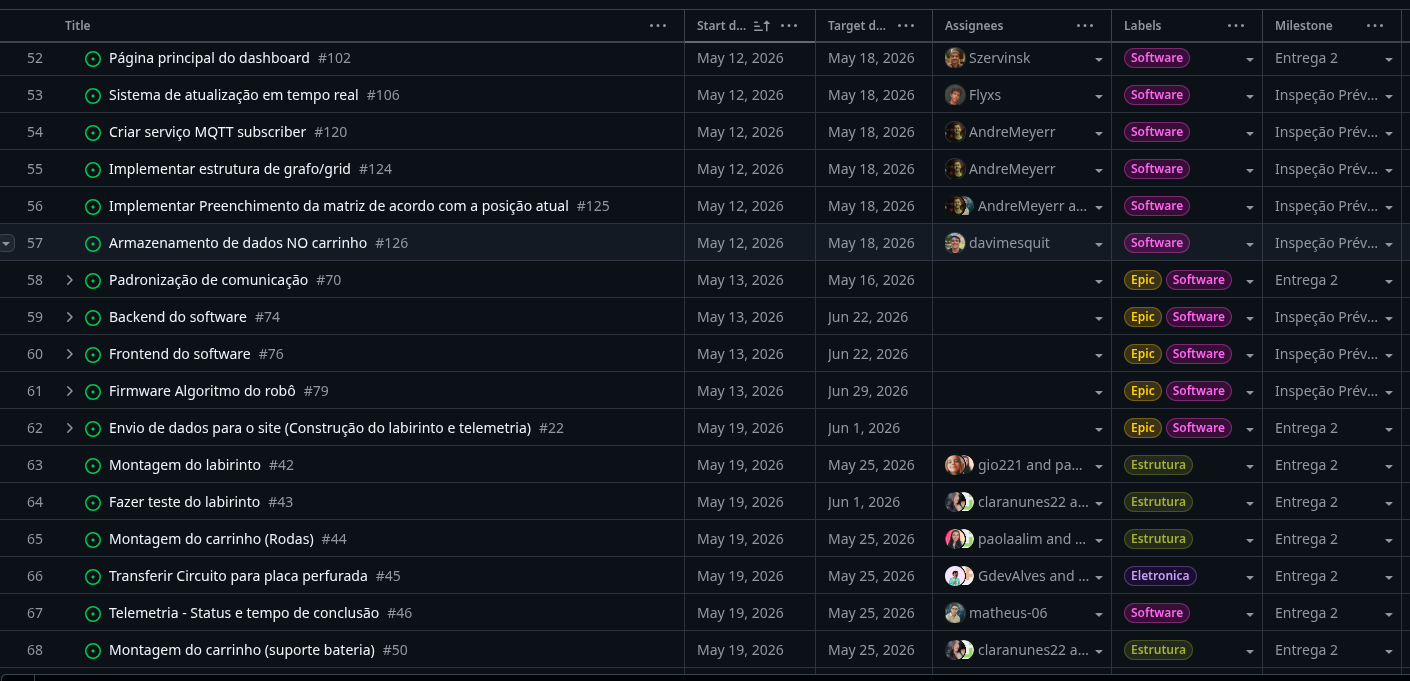
\includegraphics[width=\linewidth]{figuras/52-68.png}
    \caption{}
    \label{fig:cronograma_52_68}
\end{figure}
\end{landscape}

\begin{landscape}
\begin{figure}[H]
    \centering
    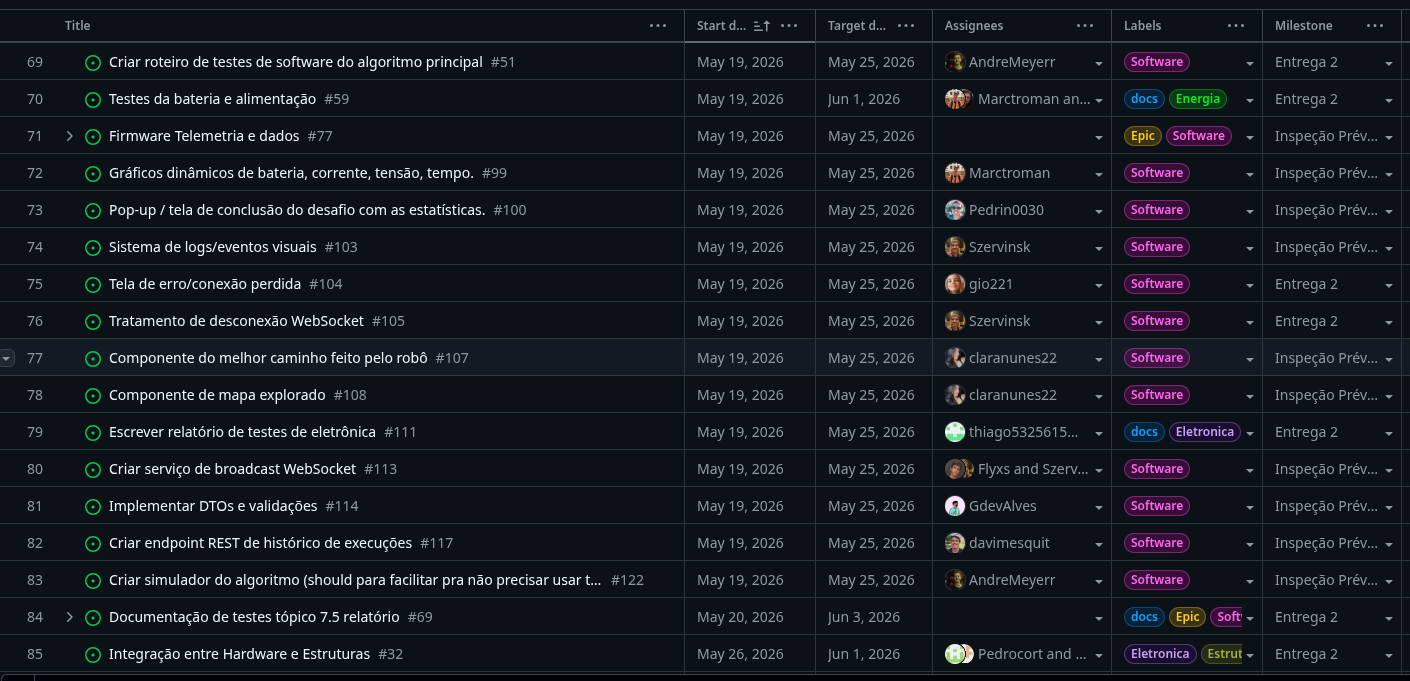
\includegraphics[width=\linewidth]{figuras/69-85.png}
    \caption{}
    \label{fig:cronograma_69_85}
\end{figure}
\end{landscape}

\begin{landscape}
\begin{figure}[H]
    \centering
    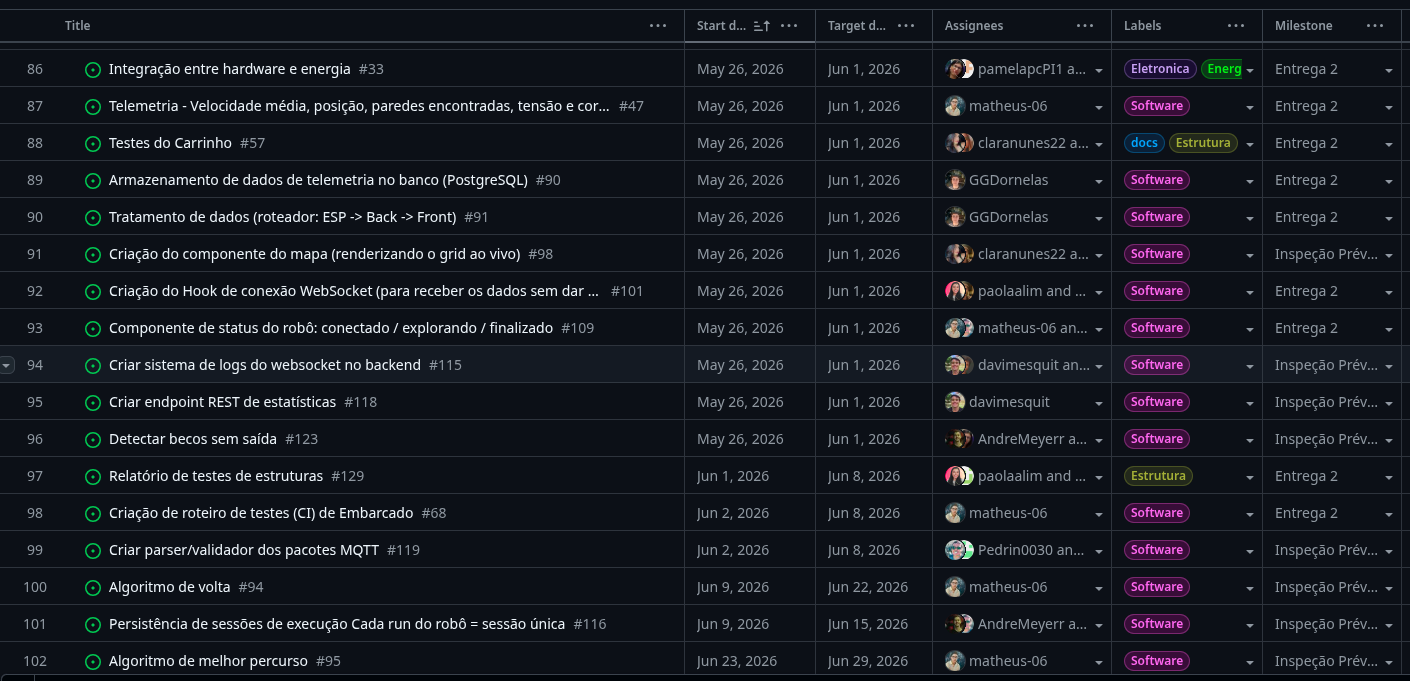
\includegraphics[width=\linewidth]{figuras/86-102.png}
    \caption{}
    \label{fig:cronograma_86_102}
\end{figure}
\end{landscape}

\begin{landscape}
\begin{figure}[H]
    \centering
    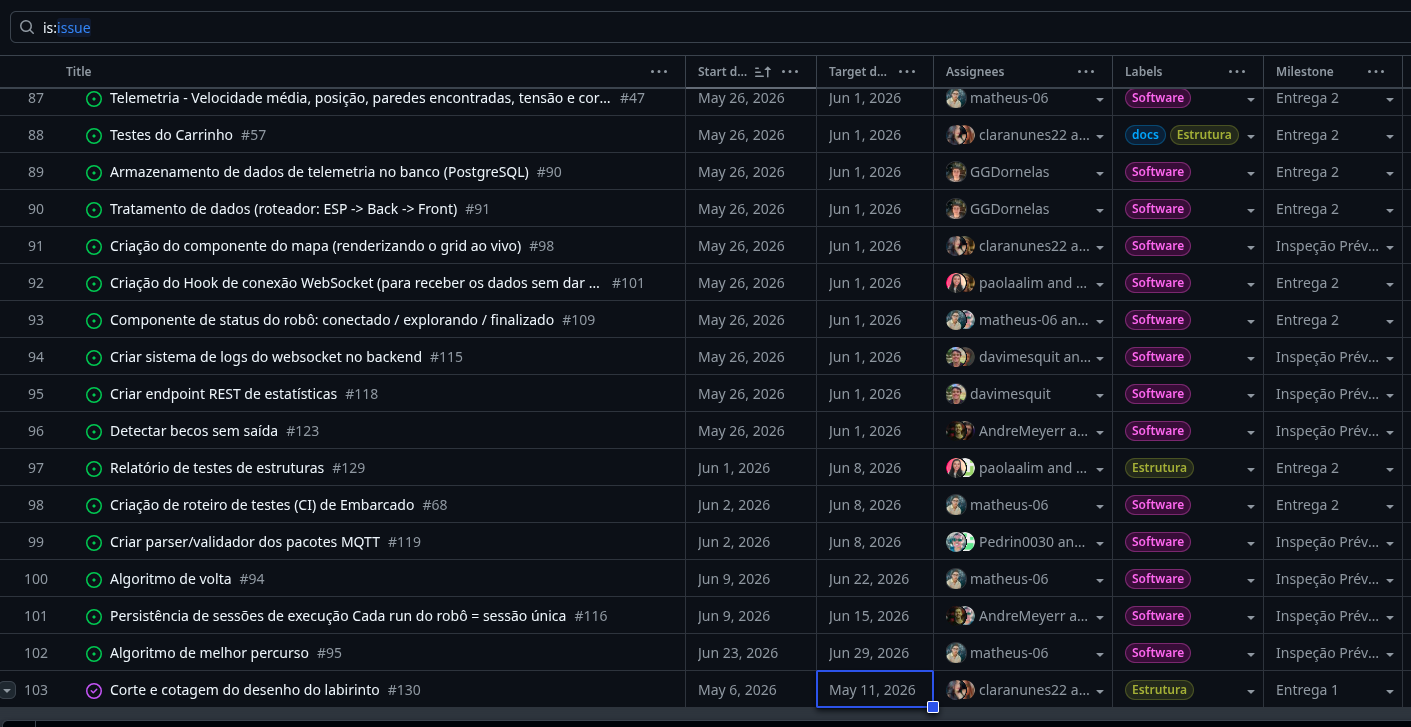
\includegraphics[width=\linewidth]{figuras/103.png}
    \caption{}
    \label{fig:cronograma_103}
\end{figure}
\end{landscape}


% \begin{table}[htpb]
% \begin{center}
% \caption{Cronograma por atividade.}
% \begin{tabular}{|c|c|c|c|c|c|c|}
% \hline
% & \textbf{Início} & \textbf{Início} & \textbf{Fim} & \textbf{Fim} & \textbf{Atividades} & \\
% \textbf{Atividade} & \textbf{Previsto} & \textbf{Realizado} & \textbf{Previsto} & \textbf{Realizado} & \textbf{Predecessoras} & \textbf{Responsáveis}\\ \hline
% 1 - ABC                       & DD/MM/AAAA               & DD/MM/AAAA                & DD/MM/AAAA               & DD/MM/AAAA                & ---                               & Fulano \\ \hline
% 2 - DEF                       & DD/MM/AAAA               & DD/MM/AAAA                & DD/MM/AAAA               & DD/MM/AAAA                & 1                                 & Fulano \\ \hline
% 3 - GHI                       & DD/MM/AAAA               & DD/MM/AAAA                & DD/MM/AAAA               & DD/MM/AAAA                & 1, 2                              & Beltrano \\ \hline
% 4 - JKL                       & DD/MM/AAAA               & DD/MM/AAAA                & DD/MM/AAAA               & DD/MM/AAAA                & 3                                 & Beltrano \\ \hline
% 5 - MNO                       & DD/MM/AAAA               & DD/MM/AAAA                & DD/MM/AAAA               & DD/MM/AAAA                & 1, 3, 4                           & Ciclano \\ \hline
% \end{tabular}
% \end{center}
% \end{table}



% \begin{table}[htpb]
% \begin{center}
% \caption{Justificativas para atrasos ou não-conclusão de atividades.}
% \begin{tabular}{|c|c|} \hline
% \textbf{Atividade} & \textbf{Justificativa}  \\ \hline 
%     3 - GHI &
%     O material solicitado não foi entregue no prazo pelo fornecedor. \\ \hline
%     5 - MNO &
%     A equipe responsável pelo desenvolvimento não finalizou a atividade. \\ \hline
% \end{tabular}
% \end{center}
% \end{table}

% %% Exemplo de tabela que ocupa várias páginas
% \begin{center}
% \begin{longtable}{|l|l|l|}
% \caption{A sample long table.} \label{tab:long} \\

% \hline \multicolumn{1}{|c|}{\textbf{First column}} & \multicolumn{1}{c|}{\textbf{Second column}} & \multicolumn{1}{c|}{\textbf{Third column}} \\ \hline 
% \endfirsthead

% \multicolumn{3}{c}%
% {{\bfseries \tablename\ \thetable{} -- continued from previous page}} \\
% \hline \multicolumn{1}{|c|}{\textbf{First column}} & \multicolumn{1}{c|}{\textbf{Second column}} & \multicolumn{1}{c|}{\textbf{Third column}} \\ \hline 
% \endhead

% \hline \multicolumn{3}{|r|}{{Continued on next page}} \\ \hline
% \endfoot

% \hline \hline
% \endlastfoot

% One & abcdef ghjijklmn & 123.456778 \\
% One & abcdef ghjijklmn & 123.456778 \\
% One & abcdef ghjijklmn & 123.456778 \\
% One & abcdef ghjijklmn & 123.456778 \\
% One & abcdef ghjijklmn & 123.456778 \\
% One & abcdef ghjijklmn & 123.456778 \\
% One & abcdef ghjijklmn & 123.456778 \\
% \end{longtable}
% \end{center}